\documentclass{article} % For LaTeX2e
\usepackage{cos424,times}
\usepackage{hyperref}
\usepackage{url}
%\usepackage{float}
\usepackage{floatrow}

\usepackage{graphicx}


\usepackage{amsmath}
\usepackage{amssymb}
\usepackage{enumerate}
%\usepackage{fullpage}
%\usepackage[margin=0.5in]{geometry}
\usepackage{bbm}

\def \mcX {\mathcal{X}}
\def \mcY {\mathcal{Y}}
\def \mcH {\mathcal{H}}
\def \mcD {\mathcal{D}}

\def \P {\mathbb{P}}

\def \N {\mathbb{N}}
\def \Nbr {\mathcal{N}}
\def \Q {\mathbb{Q}}
\def \F {\mathbb{F}}
\def \then {\implies &}
\def \oif {\Longleftrightarrow &\,}
\def \given {\text{Given }&}
\def \assume {\text{Assume }&}
\def \thfr {\therefore &\enskip}
\def \bij {\leftrightarrow}
\def \inj {\rightarrowtail}
\def \sur {\twoheadedrightarrow}
\def \Z {\mathbb{Z}}
\def \R {\mathbb{R}}
\def \C {\mathbb{C}}
\def \iff {\Longleftrightarrow}
\def \kron {\boldsymbol\delta}
\def \indicator {\mathbbm{1}}

\def\Tx{\textbf{x}}
\def\Ty{\textbf{y}}
\def\quotient{\mathclose{}/\mathopen{}}
\def\Tf{\textbf{f}}
\def\Th{\textbf{h}}
\def\Tg{\textbf{g}}
\def\sumn{\sum_{n=0}^\infty}
\def\limn{\lim_{n\rightarrow\infty}}
\def\prodn{\prod_{n=0}^\infty}
\DeclareMathOperator\adj{adj}

\newcommand{\stc}[1]{\widetilde{#1}}   
\newcommand{\pa}[1]{ \left({#1}\right) }
\newcommand{\set}[2]{ \left\{ #1 \,\middle|\, #2 \right\} }
\newcommand{\shift}[1]{&\quad & \text{#1}\\}
\newcommand{\lem}[1]{\text{\textbf{L.\ref{#1}}}}
\newcommand{\card}[1]{\left\vert{#1}\right\vert}
\newcommand{\Ps}[1]{\mathcal{P}\left({ #1 }\right)}
\newcommand{\colv}[1]{\begin{pmatrix} #1 \end{pmatrix}}
\newcommand{\mat}[1]{\begin{pmatrix} #1 \end{pmatrix}}
\newcommand{\detmat}[1]{\begin{vmatrix} #1 \end{vmatrix}}
\newcommand{\spanb}[1]{\text{span}\{ #1 \}}
\newcommand{\abs}[1]{\left|#1\right|}
\newcommand{\Inner}[1]{\langle #1 \rangle}
\newcommand{\Innercpy}[1]{\langle #1, #1 \rangle}

\DeclareMathOperator{\Err}{\text{err}}
\DeclareMathOperator*{\ErrE}{\mathbb{E}}
\DeclareMathOperator{\Tr}{tr}
\DeclareMathOperator{\Dim}{dim}
\DeclareMathOperator{\Rank}{rank}
\DeclareMathOperator{\Ker}{ker}
\DeclareMathOperator{\Diam}{diam}
\DeclareMathOperator{\Int}{int}
\DeclareMathOperator{\Clo}{clo}
\DeclareMathOperator{\sgn}{sgn}
\DeclareMathOperator{\MyRe}{Re}
\DeclareMathOperator{\MyIm}{Im}


\title{COS 424 Homework 2}

\author{
Vladimir Feinberg\\
Princeton University\\
\texttt{vyf@princeton.edu}
}

\newcommand{\fix}{\marginpar{FIX}}
\newcommand{\new}{\marginpar{NEW}}

\begin{document}

\maketitle
\begin{abstract}

We present an approach for imputing methylation values, a form of epigenetic marker, in tissue samples by relying on methylation values of other tissues and cis-regulatory genetic contexts. A combined collaborative filtering and lasso linear model approach offer an out-of-sample $R^2$ of 0.877 for predicting the methylation values of a tissue sample with only 2\% of the values known - there are a total of about 380K sites whose values must be predicted via regression for chromosome 1. Other chromosomes exhibit similar results.
\end{abstract}

\section{Introduction and Related Work}

Imputation is a general statistical process involving replacing unknown values with a best guess based on a given context. Formally, we consider some vectors $\Tx_i\in S^n$ for some set $S$. If we take these $\Tx_i$ to be sampled from a distribution over $S^n$, we can make some predictions about the posterior of a $\Tx$ given some limited observation into a set of $\{\Tx_i\}$.

In our case, $S$ is a tuple over various biological information: chromosome number, genomic offset, strand type (3'-5' or 5'-3'), and methylation, the proportion of sites in a laboratory sample that had an additional methyl group attached to a cytosine molecule. The methylation count in our data set may be missing information.

Predicting whether the proportion of methylated sites from a sample is at least half has been done with over 90\% accuracy by relying on methylation levels of nearby sites, sequence-encoded information such as genetic context, and genomic position to the extent that the site is co-located (in the binary sense) with a DNA sequence for a particular protein or a sequence for a cis-regulartory element (CRE) \cite{zhang2015predicting}. Other studies have also found co-localization between CREs and CpGs (sites where the methylation occurs) \cite{ziller2013charting}.

\section{Exploratory Data Analysis}

We focus our analysis mainly on chromosome 1, which has samples from 379551 sites. There are 34 samples for each site, each taken from an expensive WGBS procedure. This method is able to measure about 91\% of sites \cite{laird2010principles}. Our test sample only has about 2\% of the sites available from a cheaper procedure: methylation microarrays \cite{zhang2015predicting}.

We are to use the limited information to impute the missing values in the sample. Because we can only use WGBS as the true value, there are some sites that we don't know the correct value for, even in testing. The imputation procedure may {\em not} be specified to only impute the sites we are testing for because this is a facet of our testing procedure. The methods constructed attempt to impute the entire genome. We are only able to provide an estimate for our testing error because we can only observe some of the true methylation values with the more expensive technique.

The sites available at test time are consistent - the technology used to assay the methylation values samples sites consistently \cite{infinium}. This opens up opportunities to take advantage of learning patterns particular to the sites consistently tested by the methylation microarrays - for instance, we can mask one of the well-sampled tissues enabling cross-validation on a reduced feature set.

\begin{figure}[H]
    \centering
    
    \begin{minipage}[b]{0.3\textwidth}
        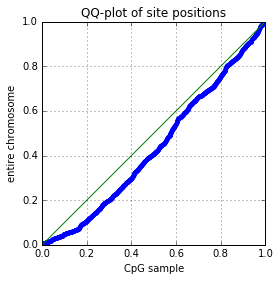
\includegraphics[width=\textwidth]{qqtest.png}
        %\caption{}
    \end{minipage}
    \hspace{0.15\textwidth}
    \begin{minipage}[b]{0.4\textwidth}
        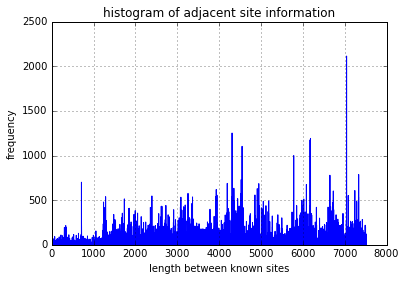
\includegraphics[width=\textwidth]{adjhist.png}
        %\caption{}
    \end{minipage}
    
    \caption{The above demonstrates the distribution of the known sites in the test sample. The mean distance between sites is 50.3, with a standard deviation of 87.0. The QQ-plot demonstrates that the sampling is fairly uniform throughout the chromosome.}
    \label{fig:sampleknowndistrib}
\end{figure}

The microarray may only provide about 2\% of the chromosome's information, but its uniformity, displayed in Figure \ref{fig:sampleknowndistrib}, coupled with the observations of correlation amongst neighboring sites from Figure \ref{fig:colocalsite}, motivates interpolation.

\begin{figure}[H]
    \centering
\floatbox[{\capbeside\thisfloatsetup{capbesideposition={left,center}}}]{figure}[\FBwidth]
{\caption{The float demonstrates estimates the correlation of methylation values with the neighbours a given distance away from a sample site on the same tissue sample. The correlation across 33 of the 34 given tissues was taken. This was performed on 1000 random sites. The last chromosome was dropped due to its 98\% sparsity. The ``bottoming out" of correlation at about 0.25 as we distance ourselves from the site matches the observed background correlation from \cite{zhang2015predicting}. Error bars are $1\hat{\sigma}$.}
    \label{fig:colocalsite}}
{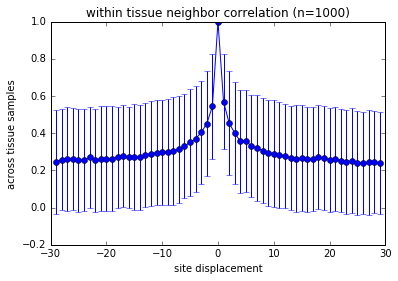
\includegraphics[width=0.4\textwidth]{colocalisitecorr.png}}
\end{figure}

We explore whether there's potential for (1) prediction based on genomic location or (2) prediction based on similarity to other chromosomes. Figure \ref{fig:genomictrends} shows the rolling mean of the methylation proportions - it confirms that while there are no obvious trends as a function of sequence, there are chromosomes with similar behavior.

\begin{figure}[H]
    \centering
    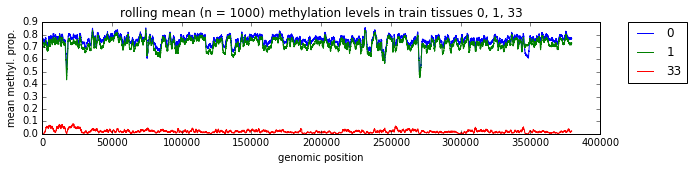
\includegraphics[width=0.9\textwidth]{genomictrends.png}
    \caption{Rolling mean with 1000 bp windows of methylation values for varying tissues. In order, the standard deviation ratio from the original tissue methylation values to the rolled mean ones are 4.83, 4.62, and 11.34. Note that this is the square root of the inverse of proportion of variance maintained by the rolling mean.}
    \label{fig:genomictrends}
\end{figure}

%TODO (once added) \CITE{} below too -> genetic context (intronic, ex, etc).
%TODO genetic context?
As recommended by \cite{zhang2015predicting}, additional info from the ENCODE project was retrieved, corresponding to the indicators that a given site is within the context of a transcription factor CRE. This introduces 161 binary features, which are used alongside the strand direction information as additional inputs compared to the other tissue methylation samples alone \cite{encode2004encode}.
\section{Methods}

Recall there are 34 sample tissues. Models were evaluated by average cross-validation performance by supplying 33 tissues with near-full methylation information and 1 sample with only the methylation sites revealed by the 2\%-sampling microarray mechanism \cite{infinium}. However, only 6 folds were performed, because certain tissue samples were sparse or highly uncorrelated with the any of the rest, and would be poor candidates for model selection for our test chromosome, see Figure \ref{fig:chromacorr}).

\begin{figure}[H]
    \centering
\floatbox[{\capbeside\thisfloatsetup{capbesideposition={left,center}}}]{figure}[\FBwidth]
{
    \caption{Using only the training data, it was found that the closest training sample was chromosome 19. Thus, we estimate from the diagram above that chromosomes 19-24, inclusive, will be good folds to use as a basis of model selection by pretending they each only have limited methylation information.}
    \label{fig:chromacorr}}
    {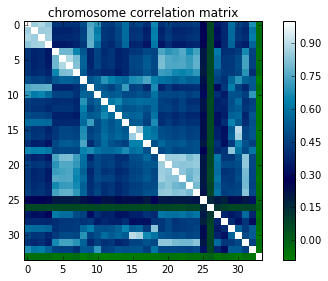
\includegraphics[scale=0.5]{chromacorr.png}}
\end{figure} 

A fundamental assumption here is that the additional tissue data at test time on the holdout tissue sample will not significantly worsen the top model from cross-validation. This is a fair assumption since the model was selected with 33 similar features.

The observations from the previous sections inform us that several approaches may be successful: interpolation between neighboring sites and identifying clusters of chromosomes according to methylation patterns. The latter has biological basis: the TA mentioned that chromosomes from the same tissue groups have similar methylation. One approach is to use our restricted amount of methylation knowledge to detect what linear combination of tissue samples, when viewed as vectors in the 380K-dimensional site space, best approximates the test sample.

There are many strategies for finding the aforementioned combination. Figure \ref{fig:chromacorr} displays several clusters - a simple approach that leverages the cluster structure is the memory-based collaborative filtering (mCF), which returns a weighted sum from the fully-assayed samples using a similarity metric defined only on the intersection of the known methylation values \cite{wiki:cf}. Similarly, we can learn this linear combination by fitting a linear model - in this case, we consider every site index a separate, independent data point, and train on the known methylation values.

Linear models considered were OLS, ridge, lasso, random forest (which is mostly linear), and elastic net. The sparse features, such as the indicators, would be harshly penalized by lasso alone. However, lasso still outperformed ridge due to its restriction of overfitting. As such, elastic net was attempted as a middle ground. Indeed, it outperformed the other models in most cases (only the best-model's CV results are displayed in the summary table, Figure \ref{fig:cvperf}).

All hyperparameter were trained on a nested 8-fold CV loop, which split the test sample's methylation sites even further for training. The ``known tissues" still had some missing samples - these were imputed with the interpolated value by neighboring sites within each individual sample. Fancier imputation was not necessary because there were so few missing sites.

\section{Results}

\begin{figure}[H]
    \centering
    \begin{tabular}{l|ccc}
method & RMSE & methylation accuracy & $R^2$ \\ \hline
local site interpolation & 0.204777 & 0.889799 & $-$0.613112 \\
within-tissue mean & 0.162478 & 0.937630 & $-$0.015392 \\
across-tissue mean & 0.131869 & 0.953696 & \phantom{$-$}0.325614 \\
1 nearest neighbor & 0.091203 & 0.968845 & \phantom{$-$}0.677763 \\
correlation mCF & 0.102694 & 0.963925 & \phantom{$-$}0.591949 \\
tissue elastic net & 0.069056 & 0.976347 & \phantom{$-$}0.814434 \\
metadata lasso & 0.154597 & 0.938605 & \phantom{$-$}0.080309 \\
neighbors lasso & 0.120148 & 0.953538 & \phantom{$-$}0.443131 \\

ensemble elastic net & 0.065382 & 0.978741 & \phantom{$-$}0.832932
\end{tabular}
        \caption{RMSE and $R^2$ values are calculated on the test data - for this reason $R^2$ is not adjusted and may also be negative. The methylation accuracy is the performance of the regression when reduced to the 0-1 classification problem for whether a site is methylated. Metadata refers to strand direction and CRE indicators. Neighbors refers to adjacent-site methylation values on different tissue samples. mCF accepts as input a similarity measure (cosine, canberra, and correlation were tested). The ensemble elastic net combines the same-site and neighbor methylation, metadata, and correlation-based mCF values as explanatory variables.}
    \label{fig:cvperf}
\end{figure} 

The three strongest non-ensemble models were combined after observation that their residuals on one of the folds are weakly correlated - the largest absolute correlation amongst the 6 pairs of predictors was 0.667, and was 0.544 on average. Taking our best best model, the ensemble lasso, and making a finer grid search based on the optimal hyperparameters from the CV yielded the results in Figures \ref{fig:finalres} and \ref{fig:finalgen}.

\begin{figure}[H]
    \centering
\floatbox[{\capbeside\thisfloatsetup{capbesideposition={left,center}}}]{figure}[\FBwidth]
{    \caption{Ensemble lasso residuals on the holdout sample. RMSE is 0.059271, methylation prediction accuracy is 0.980633, and $R^2$ is 0.877143. Note the residuals are satisfactorily normal.}
    \label{fig:finalres}}
    {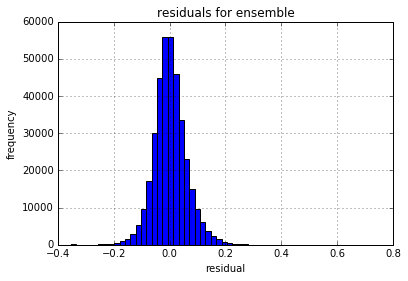
\includegraphics[scale=0.4]{ensembleres.png}}
\end{figure}

\begin{figure}[H]
    \centering
    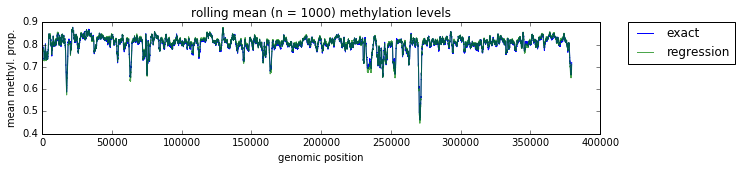
\includegraphics[width=0.9\textwidth]{ensembleseq.png}
    \caption{Rolling means of both the final regression model and the exact chromosome, with all indices included. The exact sample is still missing about 1\% of sites, which were locally interpolated for this image. The rolling mean computation reduces the variance of both sequences by at most a factor of 22.}
    \label{fig:finalgen}
\end{figure}

The entire procedure was replicated on chromosomes 2, 6, 7, and 11. This yielded test $R^2$ values of  0.871433, 0.874899, 0.870044, and 0.881261, respectively.

\section{Conclusion}

This report demonstrates the predictive power for methylation values, both individually and when combined, of memory-based collaborative filtering with a correlation-based similarity metric, CRE context indicators, and methylation values of sites in the same and neighboring positions in the genomic sequence for different tissues. The final $R^2$ of 0.877 can still be improved.

Furthermore, other methods that were either intractable or unavailable may have promise. For instance, beta regression has a more appropriate range for regression prediction. An iterative, regularized, SVD collaborative filtering algorithm may elicit different patterns than the simple memory-based one \cite{percy}.

Perhaps the most promising model that encodes all patterns that have been observed, which the author would have needed to implement in TensorFlow (but did not have time for) is a $K$-cluster GMM over the entire 380K-dimensional methylation vector of each tissue. The variance matrix would agree with our colocated correlation observations - it would be restricted to a diagonal matrix, with values for the $+i$ and $-i$ bands adjacent to the diagonal corresponding to the neighboring sites of displacement $i$. Bands with $i> A$ would be held as zero. After training for a given $K,A$, one is equipped with a mixture model over all 380K sites. This allows for a closed-form posterior given only 2\% of the sites, the mean of which may be used for prediction (and the variance for confidence). Unfortunately, the GMM built in to \texttt{scikit-learn} is not expressive enough. In addition, it was not tractable on this dataset the more naive diagonal model.


\subsubsection*{Acknowledgments}

The author would like to thank Prof. Engelhardt and Brian Jo for their advice on this project and provision of data. Also, Princeton University and the ENCODE project are responsible access to certain references and additional data sets \cite{encode2004encode}.

In addition, the author leveraged the Princeton CS Department's \texttt{cycles} systems for many of the parallelizable grid-search and preprocessing tasks.

Finally, the author heavily relied on \texttt{iPython} \cite{iPython} notebooks, \texttt{sklearn} \cite{scikit-learn} for algorithm implementations, \texttt{scipy} \cite{scipy} and \texttt{pandas} \cite{pandas} for scientific computing functions, and \texttt{matplotlib} \cite{matplotlib} for graphing.


\bibliographystyle{acm}
\bibliography{ref}

\end{document}
